
\section{Sample 04: Hidden Markov model like structure}

\begin{figure}
	\centering
\def\svgwidth{0.8 \textwidth}
\import{../src/Chapter_additional/03_Samples/image_04_05/}{HMM.pdf_tex} 
\caption{The chain structure considered by Sample 04.}
\label{fig:sample_04:0}
\end{figure}

The structure reported in Figure \ref{fig:sample_04:0} is considered in this example.
The reported chain is similar to those considered in Hidden Markov models, for which the chain of hidden variables $Y_{1,2,\cdots}$ are connected to the chain of evidences $X_{1,2,\cdots}$. The potential $\Phi_{YY0}$, represents an a-priori knowledge about variable $Y_1$. All the variables are binary and the potentials are simply correlating exponential potentials. In particular, the ones connecting the hidden variables have a weight equal to $w_{YY}$, while the ones connecting the evidences to the hidden set share a weight equal to $w_{XY}$.
The evidences are set as indicated in Figure \ref{fig:sample_04:0}, i.e. 0 and 1 are alternated in the chain represented by $X_{1,2,\cdots}$.
The MAP estimation \footnote{The Node$\_$factory class is in charge of invoking the proper version of the message passing algorithm that leads to the MAP estimation computation.} of the hidden set (Section \ref{sec:00:MAP}) is computed into two different situations:
\begin{itemize}
\item case a): $w_{XY} >> w_{YY}$
\item case b): $w_{XY} << w_{YY}$
\end{itemize}
Here the point is that when considering case a), the information about the evidences and the correlations between $Y_{1,2,\cdots}$ and $X_{1,2,\cdots}$ is predominant. On the opposite, when dealing with case b), the correlations among the hidden variables as well as the prior knowledge about $Y_0$ is predominant. For this reason, for case a) the MAP estimation of the hidden variables is equal to $h_{MAP}^a = \lbrace 0,1,0,1, \cdots  \rbrace$,
while for case b) the MAP estimation is equal to $h_{MAP}^b = \lbrace 0,0,0,0, \cdots  \rbrace$.

\section{Sample 05: Matricial structure}

\begin{figure}
	\centering
\def\svgwidth{0.55 \textwidth}
\import{../src/Chapter_additional/03_Samples/image_04_05/}{Matrix.pdf_tex} 
\caption{The matricial structure considered by Sample 05.}
\label{fig:sample_04:1}
\end{figure}

\begin{figure}
	\centering
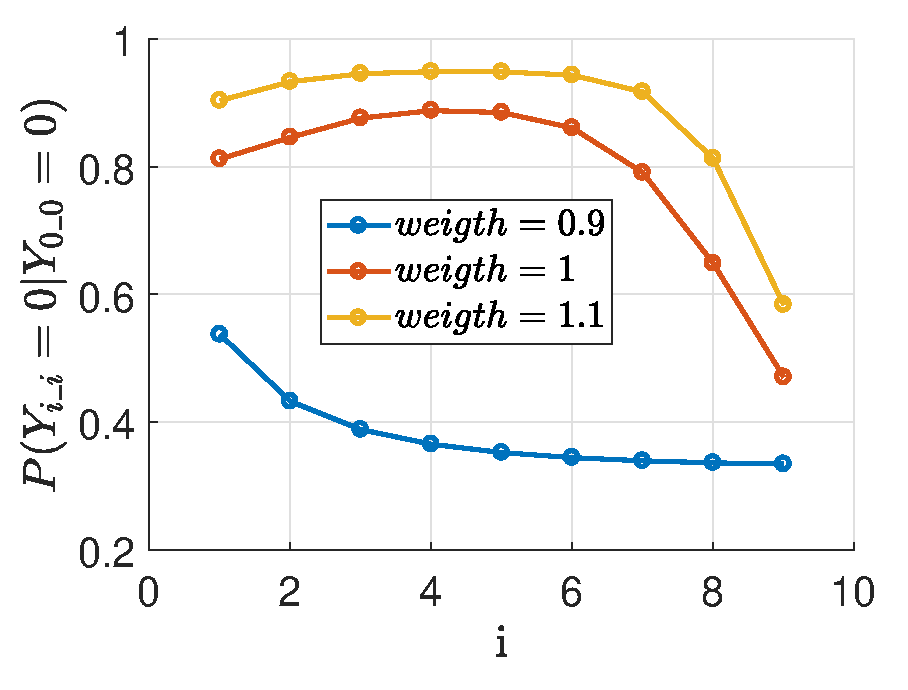
\includegraphics[width=0.48\columnwidth]{../src/Chapter_additional/03_Samples/image_04_05/Matrix_marginals.eps}
\caption{The marginals of variables $Y_{i\_i}$, conditioned to $Y_{0\_0}= 0$ as evidence of the graph reported in Figure \ref{fig:sample_04:1}, when varying the weight of the correlating exponential factors involved in the structure.}
\label{fig:sample_04:2}
\end{figure} 

The matrix-like structure reported in Figure \ref{fig:sample_04:1} is considered in this example. The variables in the matrix have all the same domain size and the are correlated by the potentials populating the matrix, which are all simple exponential correlating factors sharing the same weight.
The example builds the matrix and then assumes $Y_{0\_0} = 0$ as an evidence. Then, the marginals of the variables along the diagonal of the matrix, i.e. $Y_{i\_i}$, are evaluated. As can be seen, the marginal probability $\mathbb{P}(Y_{i\_i} = 0 | Y_{0\_0})$ decreases descending the diagonal. Figure \ref{fig:sample_04:2} reports the results obtained when varying the weight of the correlating factors, on a matrix made of $10x10$ variables having a $Dom$ size equal to $3$.